\documentclass[aspectratio=169]{beamer}

\usetheme{default}
\usecolortheme{default}
\usefonttheme{professionalfonts}
\usepackage[T1]{fontenc}
\usepackage{lmodern}
\usepackage{tikz}
\usepackage{ragged2e}
\usetikzlibrary{positioning,arrows.meta,calc,fit,shapes.geometric}

\definecolor{Navy}{RGB}{21,55,101}
\definecolor{Blue}{RGB}{32,105,168}
\definecolor{Cyan}{RGB}{25,139,158}
\definecolor{Green}{RGB}{47,126,82}
\definecolor{Orange}{RGB}{194,111,46}
\definecolor{Red}{RGB}{165,55,55}
\definecolor{Light}{RGB}{244,247,252}
\definecolor{Gray}{RGB}{82,90,103}

\setbeamertemplate{navigation symbols}{}
\setbeamertemplate{itemize item}{\color{Navy}$\blacktriangleright$}
\setbeamercolor{title}{fg=Navy}
\setbeamercolor{frametitle}{fg=Navy,bg=white}
\setbeamercolor{block title}{fg=white,bg=Navy}
\setbeamercolor{block body}{fg=black,bg=Light}
\setbeamercolor{block title alerted}{fg=white,bg=Red}
\setbeamercolor{block body alerted}{fg=black,bg=Red!7}
\setbeamerfont{frametitle}{size=\Large,series=\bfseries}
\setbeamerfont{title}{size=\LARGE,series=\bfseries}
\setbeamertemplate{footline}{%
  \leavevmode\hbox{%
    \begin{beamercolorbox}[wd=.78\paperwidth,ht=2.6ex,dp=1.15ex,leftskip=1.2em]{author in head/foot}%
      \scriptsize NDNSF-UAV: data-driven collaboration work in progress
    \end{beamercolorbox}%
    \begin{beamercolorbox}[wd=.22\paperwidth,ht=2.6ex,dp=1.15ex,rightskip=1.2em plus1fil]{date in head/foot}%
      \scriptsize \insertframenumber/\inserttotalframenumber
    \end{beamercolorbox}}}

\newcommand{\pill}[2]{\tikz[baseline=(n.base)]\node[rounded corners=2pt,fill=#1!14,text=#1,inner xsep=4pt,inner ysep=2pt,font=\scriptsize\bfseries](n){#2};}
\newcommand{\checkpill}[2]{\tikz[baseline=(n.base)]\node[rounded corners=2pt,fill=#1!14,text=#1,inner xsep=3pt,inner ysep=1.5pt,font=\tiny\bfseries](n){#2};}
\newcommand{\claim}[1]{\begin{block}{Key point}#1\end{block}}
\newcommand{\evidence}[1]{\par\noindent{\color{Gray}\tiny Evidence: #1}\par}

\title{NDNSF-UAV: Map-Selected Multi-UAV Inspection}
\subtitle{Late-bound camera UAVs capture complementary views; a selected GPU UAV analyzes them and returns named results}
\author{}
\institute{}
\date{}

\begin{document}

\begin{frame}[plain]
  \titlepage
  \vspace{-1em}
  \begin{center}
    \pill{Orange}{WORK IN PROGRESS}
    \quad\pill{Blue}{DATA-DRIVEN}
    \quad\pill{Green}{REALISTIC MVP}
  \end{center}
\end{frame}

\begin{frame}{Concrete Case: Capture, Analyze, and Display One GPS Point}
\fontsize{7.7}{8.5}\selectfont
\begin{columns}[T,onlytextwidth]
\column{.43\textwidth}
\begin{center}
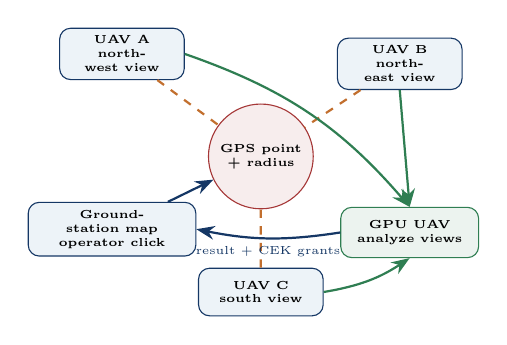
\begin{tikzpicture}[scale=.84,transform shape,
  drone/.style={rounded corners,draw=Navy,fill=Blue!8,text width=1.65cm,minimum height=.72cm,align=center,font=\tiny\bfseries},
  compute/.style={rounded corners,draw=Green,fill=Green!9,text width=1.85cm,minimum height=.76cm,align=center,font=\tiny\bfseries},
  flow/.style={-{Stealth},thick,Navy},
  data/.style={-{Stealth},thick,Green},
  sight/.style={dashed,thick,Orange}]
\node[circle,draw=Red,fill=Red!9,minimum size=1.4cm,align=center,font=\tiny\bfseries] (target) at (0,0) {GPS point\\+ radius};
\node[drone] (a) at (-2.1,1.55) {UAV A\\north-west view};
\node[drone] (b) at (2.1,1.4) {UAV B\\north-east view};
\node[drone] (c) at (0,-2.05) {UAV C\\south view};
\draw[sight] (a)--(target); \draw[sight] (b)--(target); \draw[sight] (c)--(target);
\node[rounded corners,draw=Navy,fill=Blue!8,text width=2.3cm,minimum height=.72cm,align=center,font=\tiny\bfseries] (map) at (-2.25,-1.1) {Ground-station map\\operator click};
\node[compute] (gpu) at (2.25,-1.15) {GPU UAV\\analyze views};
\draw[flow] (map)--(target);
\draw[data] (a.east) to[bend left=15] (gpu.north);
\draw[data] (b.south) -- (gpu.north);
\draw[data] (c.east) to[bend right=12] (gpu.south);
\draw[flow] (gpu.west) to[bend left=10] node[below,font=\tiny] {result + CEK grants} (map.east);
\end{tikzpicture}
\end{center}

\column{.54\textwidth}
\textbf{One concrete task}
\begin{itemize}
  \item The operator clicks a location; the planner selects three camera roles and one GPU-capable Analyzer.
  \item Each camera publishes one encrypted \texttt{ViewImage}; the Analyzer fetches admitted objects by name and processes them.
  \item The Analyzer publishes per-image annotations and requester-wrapped CEK grants. The Requester fetches the same image objects and overlays the annotations locally.
\end{itemize}
\begin{alertblock}{Why this is a realistic first case}
The known location removes target association and triangulation; the MVP reuses an existing per-view detector.
\end{alertblock}
\end{columns}
\claim{Each immutable image object serves both Analyzer and Requester; only compact annotations and recipient-bound CEK grants are newly published.}
\evidence{Multi-UAV visual inspection and coverage systems already distribute image-acquisition work across aircraft [1,2].}
\end{frame}

\begin{frame}{Fully Data-Driven NDNSF Workflow}
\fontsize{7.2}{8.0}\selectfont
\begin{center}
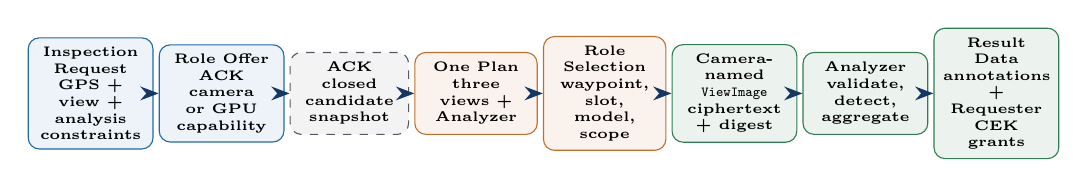
\begin{tikzpicture}[node distance=.065cm,
  discovery/.style={rounded corners,draw=Blue,fill=Blue!8,text width=1.35cm,minimum height=1.04cm,align=center,font=\tiny\bfseries},
  localbox/.style={rounded corners,dashed,draw=Gray,fill=Gray!7,text width=1.27cm,minimum height=1.04cm,align=center,font=\tiny\bfseries},
  commitbox/.style={rounded corners,draw=Orange,fill=Orange!9,text width=1.32cm,minimum height=1.04cm,align=center,font=\tiny\bfseries},
  execution/.style={rounded corners,draw=Green,fill=Green!9,text width=1.35cm,minimum height=1.04cm,align=center,font=\tiny\bfseries},
  flow/.style={-{Stealth},thick,Navy}]
\node[discovery] (request) {Inspection Request\\GPS + view + analysis constraints};
\node[discovery,right=of request] (ack) {Role Offer ACK\\camera or GPU capability};
\node[localbox,right=of ack] (close) {ACK closed\\candidate snapshot};
\node[commitbox,right=of close] (plan) {One Plan\\three views + Analyzer};
\node[commitbox,right=of plan] (selection) {Role Selection\\waypoint, slot, model, scope};
\node[execution,right=of selection] (views) {Camera-named\\\texttt{ViewImage}\\ciphertext + digest};
\node[execution,right=of views] (analyze) {Analyzer\\validate, detect, aggregate};
\node[execution,right=of analyze] (result) {Result Data\\annotations +\\Requester CEK grants};
\draw[flow] (request)--(ack); \draw[flow] (ack)--(close); \draw[flow] (close)--(plan); \draw[flow] (plan)--(selection); \draw[flow] (selection)--(views); \draw[flow] (views)--(analyze); \draw[flow] (analyze)--(result);
\end{tikzpicture}
\end{center}
\vspace{.22em}
\begin{columns}[T,onlytextwidth]
\column{.49\textwidth}
\textbf{Request and planning}
\begin{itemize}
  \item Request: point/radius, time window, view diversity, image quality, model requirement, and result deadline.
  \item Offer: cameras report reachability and view capability; processors report GPU, model, queue state, and input limits.
  \item Plan: View-A/B/C plus one Analyzer; named edges connect each View role to the Analyzer.
\end{itemize}
\column{.49\textwidth}
\textbf{Execution and result admission}
\begin{itemize}
  \item Selection assigns viewpoints and binds the Analyzer, Requester, named dependencies, model, and deadline.
  \item Each Camera publishes once under \texttt{/<camera>/NDNSF/COLLAB/...}, with request/plan/attempt, capture metadata, and a CEK wrapped to the Analyzer.
  \item The Analyzer requires prefix, signature, Plan role--Provider, and dependency-edge agreement. Its own signed result names every image/digest and carries annotations, failures, and the same CEKs rewrapped to the authorized Requester.
\end{itemize}
\end{columns}
\begin{center}
\checkpill{Blue}{ACK SNAPSHOT}\quad \checkpill{Orange}{ONE PLAN}\quad
\checkpill{Green}{REUSED VIEW DATA}\quad \checkpill{Green}{RESULT + KEY GRANT}\quad \checkpill{Red}{EXPLICIT FAILURES}
\end{center}
\vspace{-.15em}
\begin{center}\color{Navy}\bfseries The Requester fetches original images from cache or Repo, decrypts them, and overlays the returned annotations.\end{center}
\evidence{Current API: ACK closure and plan commit. In progress: cross-role input/result enforcement.}
\end{frame}

\begin{frame}{Practical Boundary, MVP, and Required Evidence}
\fontsize{7.5}{8.4}\selectfont
\begin{columns}[T,onlytextwidth]
\column{.48\textwidth}
\textbf{Responsibility boundary}
\begin{itemize}
  \item \textbf{NDNSF}: protected Request, discovery, ACK closure, producer-owned names, signer/role/dependency admission, recipient-bound CEK grants, and failure state
  \item \textbf{UAV application}: viewpoint/navigation, capture metadata, analysis invocation, annotation schema, and Requester-side overlay
  \item \textbf{Perception backend}: existing per-view detector and deterministic evidence aggregation; it does not decide Provider assignment
  \item \textbf{Autopilot}: geofence, collision, readiness, and final safety rejection
\end{itemize}
\textcolor{Red}{\textbf{Current implementation work.}} Complete dependency/result admission and Requester-bound CEK grants; integrate frame metadata and annotations.
\column{.49\textwidth}
\textbf{First measurable MVP}
\begin{itemize}
  \item one static outdoor GPS point, three camera roles, three camera UAVs, one GPU Analyzer, and one existing detector
  \item test provider unavailability, mobility, Data loss, missed deadlines, and unsafe-assignment rejection
\end{itemize}
\textbf{Measurements and ablations}
\begin{itemize}
  \item completion, valid-view and analysis success, latency, bytes, image publications per capture, and flight/energy proxy
  \item one versus three views under occlusion; nearest versus geometry-aware selection; Analyzer failure and retry
\end{itemize}
\textbf{Claim boundary}: no new recognition algorithm, moving-target identity, fleet autonomy, triangulation, or 3-D accuracy claim.
\end{columns}
\vspace{.10em}
\begin{center}\color{Navy}\bfseries End-to-end claim: each encrypted image is published once, analyzed remotely, and securely reused by the Requester.\end{center}
\evidence{[1] Mansouri et al., Control Engineering Practice 2018; [2] Luna et al., Journal of Field Robotics 2024; [3] MAVLink Common Message Set.}
\end{frame}

\end{document}
